\documentclass[12pt,a4paper]{article}
\usepackage[utf8]{inputenc}
\usepackage[spanish]{babel}
\usepackage{amsmath}
\usepackage{amsfonts}
\usepackage{amssymb}
\usepackage{makeidx}
\usepackage{graphicx}
\usepackage{lmodern}
\usepackage{kpfonts}
\usepackage{fourier}
\usepackage[left=2cm,right=2cm,top=2cm,bottom=2cm]{geometry}
\author{Rodriguez Lopez Francisco Javier}
\begin{document}

\begin{center}
\LARGE \textbf{Universidad Politecnica de la Zona Metropoilitana de Guadalajara\\}



\includegraphics[scale=1]{Upzmg3.png} 

\large \textbf{Explicacion de los Arreglos y Parametros de los Amplificadores Clase A}\\
\vspace{2cm}
\large \textbf{Nombre: Rodriguez Lopez Francisco Javier.\\
\vspace{0.5cm} Matricula: 18311804.\\
\vspace{0.5cm} Carrera: Ingenieria en Mecatronica.\\
\vspace{0.5cm} Materia: Sistemas Electronicos de Interfaz.\\
\vspace{0.5cm} Curso: septiembre-diciembre del 2019.\\
\vspace{0.5cm} Docente: Moran Garabito Carlos Enrique.}


\vspace{6cm}
\small \textbf{01 de Octubre del 2019}
\end{center}

\section{Amplificadores Clase A}\\

Este tipo de Amplificadores, su representacion, es aquel que presenta una señal con copi de la entrada pero amplificada y sin distorsion, es decir, es mejor controlada a aprtir de ondas, y señales que pueda dar este objeto, en cuanto a parametros.Este se espera que funcione en una region de parametros lineales, esto debido a su polarizacion de modo que por eso se le conoce, como amplificador clase A\\
Este en sus arreglos de potencia, su objetivo es siempre entregar su potencia de carga, el cual se considerado gracias, a si capacidad de disipar el calor, ya que sus ondas, crecen de un grado muy alto, generando asi mayor corriente, y mejor potencia en el circuito que este pueda o este trabajando.Para au mayor entendimiento, este en vez de entregar un voltaje, como lo haria cualquier carga o tension, da una mayoir señal proporcional de potencia a la carga que este va dirigido.\\

\begin{figure}[hbtp]
\caption{Amplificador tipo A}
\centering
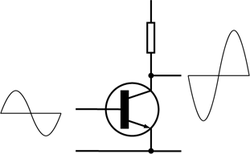
\includegraphics[width=7cm]{1.png}
\end{figure}

En este principio, es conveniente saber que los amplificadores clase A son los mas utilizados, y sencillos de entender. Se tiene que tomar en cuenta que el nucleo del amplificador calse A, es un transistor, en funcion de corte, en temas se puede explicar que este tipo de transitores, trabaja de mejor forma con resistencias a los costados del conector y el emisor, y una en paralelo de ello, esto para que el disparo de potencia, sea la mitad de la potencia obteniendo una amplitud, y esta polarizado, quedando en el punto Q.\\

Ahora para poder entenderlo mejor, si este es manipulado desde la entrada de la carga, al principio del circuito o de las conexiones que este tenga, en conjunto con los componenetes, obtendremos un mayor voltaje, y un menor voltaje, esto dependiendo de que tan brusco sea el disparo de potencia, en este caso, las ondas que se pueden presentar( en casos mas particulares, senoidales), sus ondas se incrementan en un tamaño considerable cambiando de 5v a 7v, esto por la entrada del conector disipada en el nucleo del amplificador.\\

Un  punto a considerar de sus parametros, es que este al tener resistencias conectadas en su nucelo, lo que hara este es empezar con una entrada de señales en el rango positivo, pero cuando este llega a su punto del emisor y conector, lo que hacen esas resistencias, es invertir esa onda, pero con generaciones mas grande de potencia, haciendo el cambio de voltaje, esto depende el calculo que tu manipules para la realizacion de esto, no importa si la informacion de la onda, sale disipada para arriba o para abajo, la informacion no cambia y eso es lo que nos interesa. Que llega al limite de la carga directa, ya sea este el voltaje directo, que te demande las conexiones.\\

\begin{figure}[hbtp]
\centering
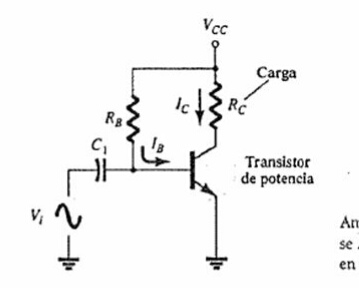
\includegraphics[width=8cm]{2.jpg}
\caption{Conexion en conector}
\end{figure}

Notas de los amplificadores de esta clase, es que siempre estaran trabajando su voltaje, sin parar, pero cuando el incremento de votaje llega a un punto en el que pasando por el nucleo, lo que hace es llegar a su limite, el limite que tu condicionaste para ello, en este caso, las ondas (si son senoidales), estaran como en pausa dentro de un periodo de pausa, tanto parte negativa, como positiva, esto debido a que el amplificador, llego a un punto en el que aunque el te quiera proporcionar mas, no podra debido a que esta fuera de rango. Entonces entramos a temas, en los que no se puede inventar un voltaje negativo, ya que los factores no estan dentro de ello.\\
LLegando a esto se tiene que tener cuidado, ya que el amplificador no estara trabajando su carga de forma lineal en todo momento, esto hara que su funcion se cumpla de una forma armonica mayor, distorcionando el principio de los amplificadores, y de su funcion.\\

\begin{figure}[hbtp]
\centering
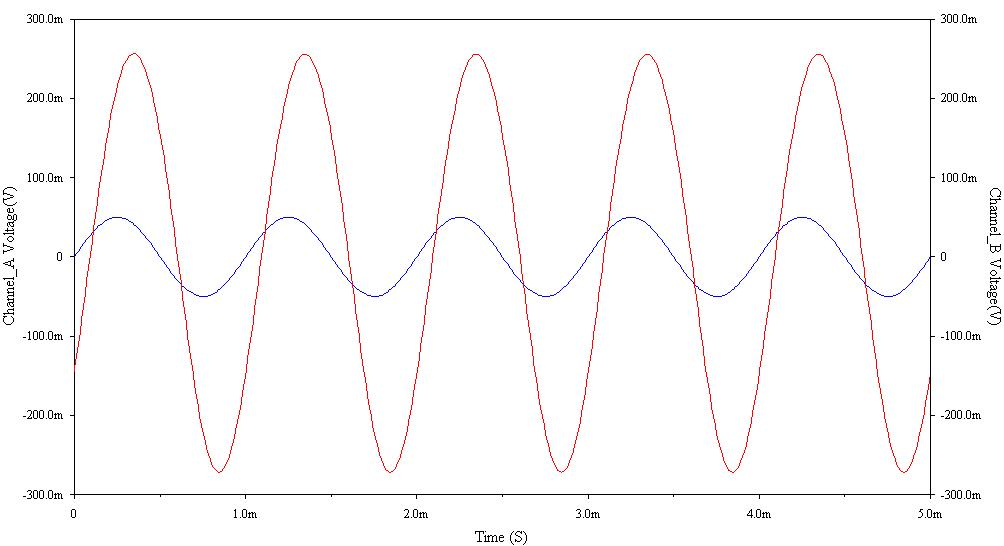
\includegraphics[width=7cm]{4.jpg}
\caption{Ondas de amplitud}
\end{figure}

En otro caso particular, si las conexiones de las resistencias en este caso estan unicamente en el conector del nucleo, esto lo que hara es trabajar simplemente con una parte de la fuente de aliemnatcion, menor a la de entrada, entonces las ondas generadas en este punto no estaran a la mitad, como se esperaria sino que estaran trabajando por debajo de la mitad, topando continuamente con el 0 de la carga, lo mismo pasa si el voltaje llega a un punto en el que sobrepasa la entrada de carga, llegando a topar pero en este caso con el maximo de potencia requerida en las conexiones. Llegando a esto, sus parametros pueden ser definidos.\\

\begin{figure}[hbtp]
\centering
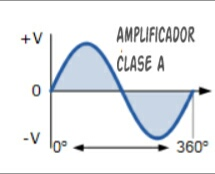
\includegraphics[width=8cm]{3.jpg}
\caption{Amplitud tipo A}
\end{figure}

\textbf{Parametros:}\\
1-Donde su amplitud de onda, es mayor a la inicial.\\
2-En una amplitud de onda reflejada en la entrada.\\
3-Amplitud de la onda es incidente en la salida.\\
4-Asi como su onda es reflejada en la salida.\\
5-Tener a consideracion, los valores de resistencias a conectar.\\
6-Donde la Energia esta dispada por la potencia.\\
7-LImite de voltaje llegado a cero hasta su maximo.\\

Entonces si con el amplificador tipo A, solo podemos modificar la alimentacion que tenemos, porque no hacerlo de mayor rendimiento y trabajo, esto es la diferencia entre un amplificador tipo A y tipo B, ya que este tiene integrado un transistor de mas, siendo estos complementarios uno del otro, para que estos sean un NP y un PNP, entonces las  ondas generadas por este tipo de amplificadores, se queda expresado por el superamiento de un voltaje que seria en eficiencia los 0.6v, sobrepasando este limite, el primer transistor se abre, generando que alimente lo que se quiera alimentar ya sea de ello una resistencia que genere la salida de audio o video, o en otro caso una bobina, el cual hace mejor su uso en amplitud de voltaje y subjetividad de ello, es la inferencia que hay entre un amplificador y otro, siendo este mayor complemento, para otro punto de partida, en el cual los dos nucleos a paritr de uno del clase A, sea establizado de mejor forma y mayor control de potencia y amplitud.\\

\begin{figure}[hbtp]
\centering
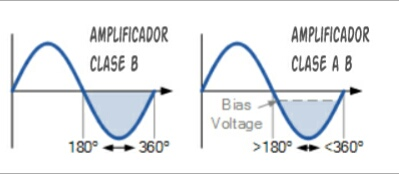
\includegraphics[width=8cm]{5.jpg}
\caption{Ondas de amplitud tipo A y B}
\end{figure}


Trabajando uno del otro, cuando este supera los 0,6v, se puede trabajar de mejor forma dada polaridad positiva del amplificador, o en otro caso, que este no supere los 0,6v, lo que pasa en este caso, es que trabaja pero con la informacion del lado negativo, este en cambio al tipo A, no trabaja con ondas senoidales, sino que trabaja de negativo a positivo, su primordial parametro es superar o inferir en los 0,6v, que es el control en donde se queda la utilizacion para que el pirmer transistor este abierto y el otro en amplitud, o viceversa.

\textbf{Referencias Bibliograficas:}

https://www.youtube.com/watch?v=3FVnao-K2_k
\end{document}